\chapter{Clustering}\label{sec:clustering}

\newcommand{\cost}{\mathcal{C}\textit{ost}}

Clustering is a name that refers to a broad class of problems that involve sets of objects, usually modeled as points in a multidimensional space, with a notion of distance between each other; the goal is to group all the points in \emph{clusters} such that the given definition of distance is minimized among the points in each cluster, and maximized between points of different clusters.

While the number of clusters need not be fixed, in some traditional approaches it is indeed fixed at a given value $k$; there are three widely known variants of clustering that are grouped together in what is called \emph{centroid-based clustering}:
\begin{itemize}\label{clust-k-algs}
    \item \textit{k-medians}: find the location of the $k$ centers as to minimize the average distance between a point and a center;
    \item \textit{k-centers}: find the location of the $k$ centers as to minimize the maximum distance between a point and a center;
    \item \textit{k-means}: find the location of the $k$ centers as to minimize the square of the distance between a point and a center. This is the most used in practice because its objective functions resemble probability variance, thus it can be interpreted as the search of Gaussian distributions that randomly generate the points of the original dataset.
\end{itemize}

\begin{example}
    Consider a product delivery company having a dataset of users, each one with their geographic position in a map. The company has a large enough budget to deploy $k$ warehouses, and its goal is to find the best places to build them. A reasonable strategy would be to apply the \emph{k-medians} model, with the intent of minimizing the average distance between a user and its closest warehouse, therefore minimizing average delivery times.
\end{example}

\begin{example}
    Consider a social network memorized as a dataset, where each user is modeled as a vector. Social networks of some significance are expected to contain billions of users, and each user's vector could have up to millions of dimensions.\footnote{this phenomenon is aptly named the \emph{curse of dimensionality}, of which an introduction can be found \href{https://en.wikipedia.org/wiki/Curse_of_dimensionality}{here}}
    The distance between any two users might reveal how much they are similar, based on the assumption that friends share common interests; an efficient way to advertise specific products would be to group users in friendship clusters, and simply target specific ads to a whole cluster.
\end{example}

Generally, centroid-based clustering problems are known to be \np-complete. In some real case studies, the number of clusters is not explicitly set, and other formulations like \textit{hierarchical clustering} are used. However, this technique produces only some levels of grouping; at some point, a decision about how many clusters are needed has to be made, and such a decision might not always have a trivial answer. An example of such conundrum is shown in figure \ref{fig:hierarchical-clustering-ex}, where either one of the three clustering levels is deemed acceptable, or a different, intermediate number of clusters is preferred, and thus another run of the hierarchical clustering algorithm is needed.
    
\begin{figure}[ht]
    \centering
    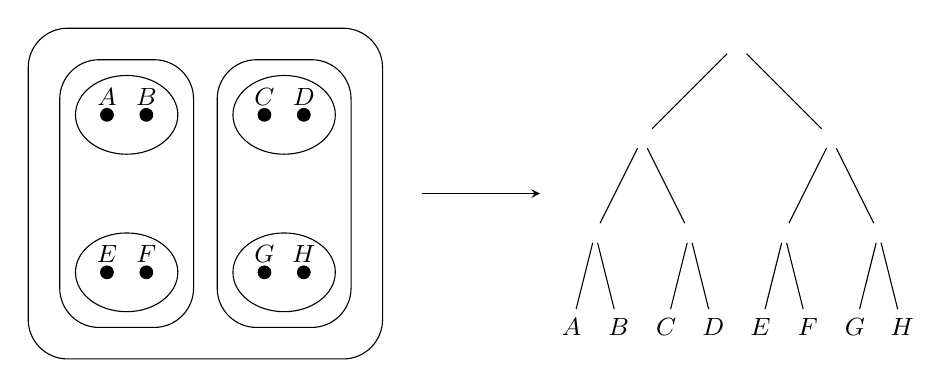
\begin{tikzpicture}[font = \small]
        \draw [fill]
            (0, 0) circle [radius = 0.8mm, fill, outer sep = 0.5mm] node [above] {$A$}
            (0.5, 0) circle [radius = 0.8mm, fill, outer sep = 0.5mm] node [above] {$B$}
            (2, 0) circle [radius = 0.8mm, fill, outer sep = 0.5mm] node [above] {$C$}
            (2.5, 0) circle [radius = 0.8mm, fill, outer sep = 0.5mm] node [above] {$D$}
            (0, -2) circle [radius = 0.8mm, fill, outer sep = 0.5mm] node [above] {$E$}
            (0.5, -2) circle [radius = 0.8mm, fill, outer sep = 0.5mm] node [above] {$F$}
            (2, -2) circle [radius = 0.8mm, fill, outer sep = 0.5mm] node [above] {$G$}
            (2.5, -2) circle [radius = 0.8mm, fill, outer sep = 0.5mm] node [above] {$H$}
        ;

        \draw
            (0.25, 0) ellipse [x radius = 0.65, y radius = 0.5] {}
            (2.25, 0) ellipse [x radius = 0.65, y radius = 0.5] {}
            (0.25, -2) ellipse [x radius = 0.65, y radius = 0.5] {}
            (2.25, -2) ellipse [x radius = 0.65, y radius = 0.5] {}
        ;
        
        \draw [rounded corners = 5mm]
            (-0.6, 0.7) rectangle (1.1, -2.7)
            (1.4, 0.7) rectangle (3.1, -2.7)

            (-1, 1.1) rectangle (3.5, -3.1)
        ;

        \draw[->, > = stealth] 
            (4, -1) -- (5.5, -1)
        ;
        
        \path [level distance = 1.2cm,
                level 1/.style = {sibling distance = 2.4cm},
                level 2/.style = {sibling distance = 1.2cm},
                level 3/.style = {sibling distance = 0.6cm}]
            (8, 0.9) node {} 
                child{ node {}
                    child{ node {}
                        child { node {$A$} }
                        child { node {$B$} }
                    }
                    child{ node {}
                        child { node {$C$} }
                        child { node {$D$} }
                    }
                }
                child{ node {}
                    child{ node {}
                        child { node {$E$} }
                        child { node {$F$} }
                    }
                    child{ node {}
                        child { node {$G$} }
                        child { node {$H$} }
                    }
                }
        ;
    \end{tikzpicture}
    \caption{An example of hierarchical clustering.}
    \label{fig:hierarchical-clustering-ex}
\end{figure}

On a theoretical standpoint, if $k$ is left unspecified, there are solutions that are trivially optimal, but have no practical use: if the goal is to minimize the distance within clusters, then the optimal solution is the singleton partition, whereas if the goal is to maximize the distance among clusters, then the optimal partition is indeed the trivial one. A technique called \textit{correlation clustering} has been designed that overcomes this limitation.


\section{Correlation clustering}\label{sec:corr-clust}

In the correlation clustering model, the graph of interest is modeled as a complete undirected graph $\mathcal{K}_n$, where all edges are partitioned into two classes $E^+$ and $E^-$. Each edge lies in either one of the two classes according to a metric $d$ operating on the vertices of $G$: if the endpoints of an edge are similar by the metric, then the edge lies in $E^+$, otherwise it is in $E^-$. An alternative, equivalent perspective is to consider a generic undirected graph as the starting model, and viewing $E^+$ as its set of edges, and $E^-$ as all the other edges that are missing.
The goal of putting similar nodes together and different nodes separated becomes for all clusters in a clustering $T$, to maximize edges from $E^+$ and minimize those from $E^-$ inside them. This notion is formalized by the function $\cost$:

\begin{equation}\label{eq:clust-cost}
    \cost(T) = \sum_{\{i, j\} \in E^+} \left[ \nexists S \in T : i, j \in S \right] + \sum_{\{i, j\} \in E^-} \left[ \exists S \in T : i, j \in S \right]
\end{equation}

Note that a clustering result $T$ is indeed a partition of the vertices $V$, with the added quirk that it will never contain an empty set.

\begin{example}
    Consider the example of correlation clustering in picture [\ref{fig:corr-clustering-ex}], where negative edges are dashed. In all the figures throughout this chapter, if an edge is either dashed or missing, then it is assumed to be in $E^-$. In this case, the nodes $A$, $B$, $C$ and $D$ are grouped together in cluster $C_1$ and the node $E$ is left alone in cluster $C_2$, since the first nodes are all similar to each other, while the other is dissimilar from all the others.
    
    \begin{figure}
        \centering
        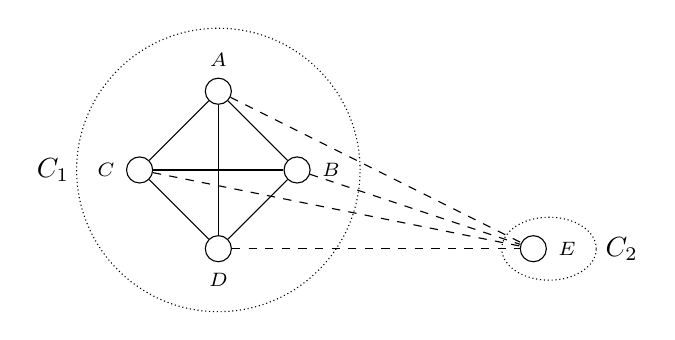
\begin{tikzpicture}
            \draw
                (0, 0) node (a) [draw, circle] {} node [above, outer sep = 2mm, font = \scriptsize] {$A$}
                (1, -1) node (b) [draw, circle] {} node [right, outer sep = 2mm, font = \scriptsize] {$B$}
                (-1, -1) node (c) [draw, circle] {} node [left, outer sep = 2mm, font = \scriptsize] {$C$}
                (0, -2) node (d) [draw, circle] {} node [below, outer sep = 2mm, font = \scriptsize] {$D$}

                (4, -2) node (e) [draw, circle] {} node [right, outer sep = 2mm, font = \scriptsize] {$E$}

                (a) edge (b)
                (a) edge (c)
                (a) edge (d)
                (b) edge (c)
                (b) edge (d)
                (c) edge (d)
                
                (a) edge [dashed] (e)
                (b) edge [dashed] (e)
                (c) edge [dashed] (e)
                (d) edge [dashed] (e)
            ;

            \draw[densely dotted]
                (0, -1) circle [radius = 1.8] (-2.1, -1) node {$C_1$}
                (4.2, -2) circle [x radius = 6mm, y radius = 4mm] (4.6, -2) node [right, outer sep = 2mm] {$C_2$}
            ;
        \end{tikzpicture}

        \caption{An example of correlation clustering.}
        \label{fig:corr-clustering-ex}
    \end{figure}

\end{example}

Optimal solutions are thus easy to find if the graph consists of disjoint cliques: the cliques themselves make a perfect clustering, with zero cost. The practical implication is that, on instances that do have a zero cost solution, a multiplicative approximation is possible only if an algorithm always finds it; otherwise the approximation will be infinite, even if the cost is small.

Of course, this is not the general case; indeed most instances do have a minimum cost for clustering, the simplest one being a graph of three vertices with two edges. Figure \ref{fig:clust-special} shows all possible clustering options of such a graph, and it should be clear that none of them have zero cost; for this reason, this particular graph is called a \emph{bad triangle}. Further considerations are made on graphs that are made by composing two triangles: if they share the middle vertex, each still has a minimum cost of 1, while if they have a common positive edge, the singular cost drops to $\half$; figure \ref{fig:clust-bad-triangles} shows this, highlighting the bad triangles involved.

\begin{figure}
    \centering
    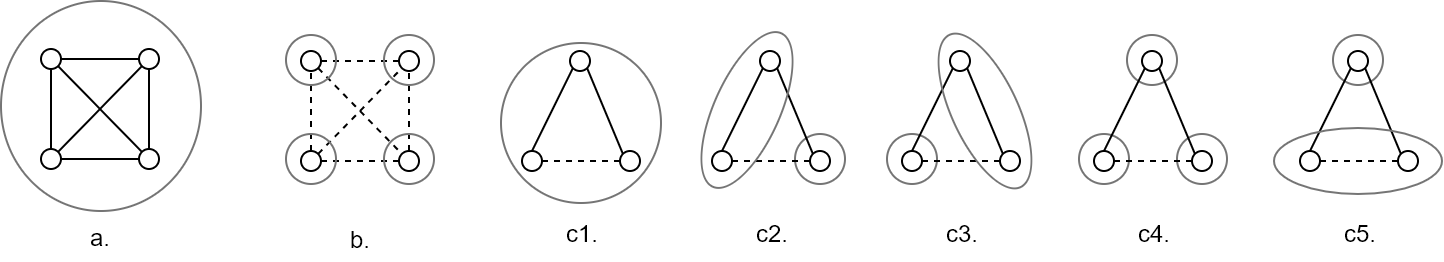
\includegraphics[width=\textwidth]{clust-special}
    \caption{Special cases in correlation clustering.}
    \label{fig:clust-special}
\end{figure}

\begin{figure}
    \centering
    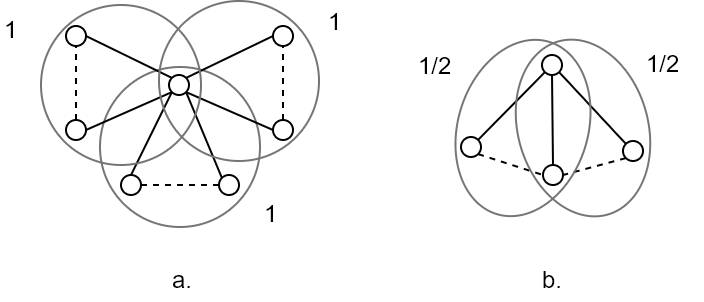
\includegraphics[width=\textwidth]{clust-bad-triangles}
    \caption{Cost of bad triangles.}
    \label{fig:clust-bad-triangles}
\end{figure}

Rather surprisingly, it can be shown that the minimum cost for clustering a graph can be related with good accuracy to how many bad triangles the graph contains as subgraphs. This motivates a formalization:

\begin{definition}[Bad triangle]
    Let $\mathcal{K}_n$ be a complete graph with its edges partitioned into two disjoint subsets $E^+$ and $E^-$. The family $G_\triangle$ collects all the bad triangles of $G$:
    \[
        G_\triangle = \{ \{x, y, z\} \subseteq V(G) : \{x, y\}, \{y, z\} \in E^+ \wedge \{x, z\} \in E^-\}
    \]
\end{definition}


\subsection{Randomized pivot}\label{sec:random-pivot}

This is an approximation algorithm for solving the correlation clustering problem designed by Ailon, Charikar, Newman:
\begin{lstlisting}[caption = {Randomized Pivot algorithm}, label = {lst:clust-random-pivot}]
algorithm $\rpgre(V, E^+, E^-)$:
    $T \gets \emptyset$
    while $V \neq \emptyset$:
        $v \pickUAR V$                                      // pick a pivot 
        $C \gets \left\{ w \in V : \{v, w\} \in E^+ \right\} \cup \{v\}$   // create a new cluster $C$
        $T \gets T \cup \{C\}$
        $V \gets V \setminus C$                              // remove all the nodes of $C$
    return $T$
\end{lstlisting}

\begin{example}
    Here is a collection of correlation clustering instances, along with solutions provided by the Randomized Pivot algorithm. In figure \ref{fig:clust-rp-1}, on the left, the algorithm provides a good approximation of an optimal solution: an improvement would be to split $C_1$ into two more components, one of them holding a bad triangle; this would reduce the cost by $1$. The right diagram shows that, if a zero cost solution exists, the algorithm reliably succeeds in finding it.\footnote{This can be proven by observing that in cliques, all vertices are adjacent to each other, a property exploited by $\rpgre$}
    
    \begin{figure}[ht]
        \centering
        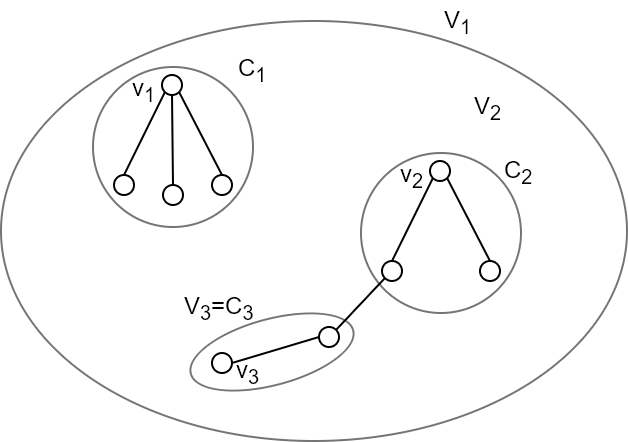
\includegraphics[width=0.45\textwidth]{clust-rp-1}
        \hspace{1pt}
        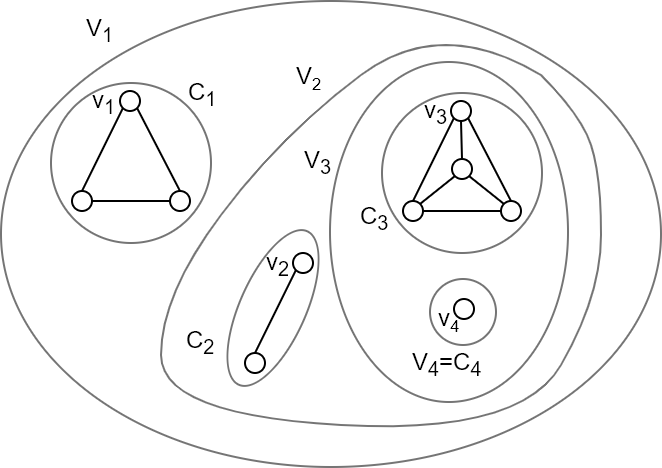
\includegraphics[width=0.45\textwidth]{clust-rp-2}
        \caption{Two runs of Randomized Pivot on different graphs: the left one does not have a zero cost solution}
        \label{fig:clust-rp-1}
    \end{figure}

    In figure [\ref{fig:clust-rp-3}] is a case in which the algorithm potentially provides a very bad approximation: if the graph is a star, there are two possible outcomes:
    \begin{itemize}
        \item the algorithm picks a leaf as a pivot, and the cost of the resulting solution will be $n - 1$;
        \item the algorithm picks the root as a pivot, and the cost will grow up to $\binom{n-1}{2} \approx n^2$. Note that picking the root \uar{} happens with probability $\oneover{n}$, which might not be as negligible as desired.
    \end{itemize}
    
    \begin{figure}
        \centering
        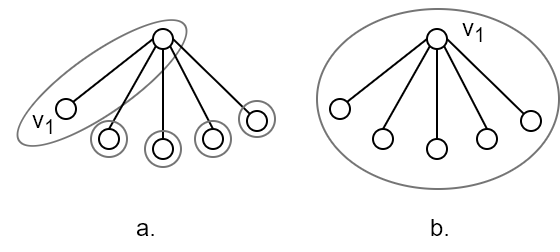
\includegraphics[width=0.5\textwidth]{clust-rp-3}
        \caption{Worst case of approximated solution of Randomized Pivot.}
        \label{fig:clust-rp-3}
    \end{figure}    
\end{example}

Despite some pathological cases such as a star graph, this algorithm does yield good approximations on average:

\begin{theorem}\label{thm:clust-rp-approx}
    Randomized Pivot [\ref{lst:clust-random-pivot}] returns on average a 3-approximation of an optimal solution:
    \[
        \expect(\cost(\rpgre(G))) \leq 3 \cdot OPT_\textsc{cc}.
    \]
\end{theorem}

\begin{obs}\label{obs:clust-4}
    By using Markov Inequality [\ref{eq:markov}], it can be proved that the bad event have small probability, if we execute the algorithm many times:
    \begin{itemize}
        \item Let $X=cost(\mathscr{C})$, $X$ is a not concentrated random variable with expected value $E[X] \leq 3 \cdot OPT$;
        \item $\Pr{X \geq 3 \cdot c \cdot OPT} \leq \Pr{X \geq c \cdot E[X]} \leq \frac{1}{c}$;
        \item If we pick $c=1+\frac{\varepsilon}{3}$, then $\Pr{X \geq (3 + \varepsilon) \cdot OPT} \leq \frac{1}{1 + \varepsilon / 3} = 1 - \Theta(\varepsilon)$;
        \item Thus, if we execute the algorithm $\frac{1}{\Theta(\varepsilon)}$ times, the probability of the bad event becomes small:\\
        $\left( 1 - \Theta(\varepsilon) \right)^{\left( \frac{\ln 1/\delta}{\varepsilon} \right)} \to \Theta(\delta)$;
        \item At this point, it is sufficient to return the best solution among those computed by the algorithm in the various trials, and with high probability it will be a solution that respects the 3-approximation, that is, a solution for which the bad event doesn't happen.
    \end{itemize}
\end{obs}

\begin{proof}[Proof of Theorem \ref{thm:clust-rp-approx}]
    Recall the definition \ref{eq:clust-cost} of the cost function; there are two sums added together:
    
    \begin{itemize}
        \item one sum involves edges in $E^+$, where the cost for one edge is $1$ whenever its endpoints lie in different clusters. In terms of the algorithm, this can be expressed in an equivalent manner as saying that, given the first cluster $C^{(i)}$ that captures one of the two endpoints $x$, the other endpoint $y$ will not be pulled into $C^{(i)}$, and thus appear in the next iteration inside $V^{(i + 1)}$:\footnote{Another implication is that $x$ cannot be a pivot}
        \[
            \left[ \nexists i : x, y \in C^{(i)} \right] \iff \left[ \exists i : x \in C^{(i)} \wedge y \in V^{(i + 1)} \right]
        \]
        \item the other sum involves edges in $E^-$, each contributing to the cost when its own endpoints belong to the same cluster. Algorithmically, this translates as saying that for each edge with cost $1$, at some iteration $i$, the relative cluster $C^{(i)}$ will capture both endpoints at the same time:\footnote{Also, neither endpoint can be a pivot}
        \[
            \left[ \exists i : x, y \in C^{(i)} \right]
        \]
    \end{itemize}

    Let $\cost_+^{(i)}$ and $\cost_+^{(i)}$ be the costs that incur respectively for cutting positive edges and from preserving negative edges on an arbitrary iteration $i$, with the single edge cost expressed algorithmically as above. Given a solution $T$ returned by the algorithm $\rpgre$, its total cost can be rewritten as follows:
    \[
        \cost(T) = \sum_{i \in \textsc{iter}} \cost_+^{(i)} + \sum_{i \in \textsc{iter}} \cost_-^{(i)}
    \]

    These costs are directly linked to specific bad triangles:
    
    \begin{claim}\label{cl:clust-1}
        $\cost_+^{(i)}$ is the number of bad triangles $T$ for which there exists an iteration $i$ such that:
        \begin{enumerate}
            \item $T$ contains $v^{(i)}$,
            \item $C^{(i)}$ contains exactly two vertices of $T$,
            \item $V^{(i)}$ includes $T$.
        \end{enumerate}
    \end{claim}

    \begin{claim}\label{cl:clust-2}
        $\cost_-^{(i)}$ is the number of bad triangles $T$ for which there exists an iteration $i$ such that:
        \begin{enumerate}
            \item $T$ contains $v^{(i)}$,
            \item $C^{(i)}$ includes $T$.
        \end{enumerate}
    \end{claim}

    \begin{definition}[Hit]\label{def:clust-hit}
        It is said that an instance of Randomized Pivot \emph{hits} a bad triangle $T$ if there is an iteration $i$ such that $V^{(i)}$ includes $T$, and the pivot $v^{(i)}$ is among the vertices of $T$.
    \end{definition}

    \begin{corollary}\label{cor:clust-1}
        For any solution $H$ given by the algorithm, $\cost(H)$ is the number of bad triangles hit by the algorithm during execution.
    \end{corollary}

    \begin{proof}
        Follows by the claims [\ref{cl:clust-1}] and [\ref{cl:clust-2}] and by definition [\ref{def:clust-hit}].
    \end{proof}
    
    We introduced the concept of \textit{hitting} because we want to relate the probability of hitting a bad triangle with the cost paid by the algorithm. We can't directly compute this probability, but we obtain a useful linear relationship.
    \begin{lemma}\label{l:clust-2}
        Given an instance of correlation clustering, for each bad triangle $T \in G_\triangle$ let $p_S$ be the probability of the Randomized Pivot algorithm hitting it.\footnote{Care should be taken while thinking about such probabilities, as which triangle gets hit or not, and how probable are such events on any specific itertion generally depends on the previous random choices the algorithm makes} Then:
        \[
            \expect(\cost(\rpgre(G))) = \sum_{T \in G_\triangle} p_T
        \]
    \end{lemma}

    \begin{proof}
        Lemma [\ref{l:clust-2}] follows by Corollary [\ref{cor:clust-1}] and the definition of expected value [\ref{def:expected-value}]: we know that $cost(\mathscr{C}_G)$ is a random variable (it depends on $\mathscr{C}_G$, that is the result returned by Randomized Pivot, that in turn is a random algorithm, as the name suggests), and, since its value is the number of bad triangles hit by the algorithm, we can decompose it in a sum of Bernoulli random variables $X_T$, one for each $T \in G_\triangle$, that assume value 1 if the algorithm hits $T$, with probability $p_T$, and 0 otherwise.
    \end{proof}

    So, finally we have all the tools we need to prove that $E\left[cost\left( \mathscr{C}_G \right)\right] \leq 3 \cdot OPT$ (the claim of Theorem [\ref{thm:clust-rp-approx}]), that is, $\frac{\sum_{T \in G_\triangle} p_T}{3} \leq OPT$, and we'll do it with a primal-dual proof, exploiting the linear program underlying Randomized-Pivot.
    
    This is a dual \lp{} formulation of the correlation clustering problem:
    
        \begin{align*} \label{lp:clust-dual}
            & \min \left( \sum_{\{i, j\} \in E(G)} X_{\{i, j\}} \right) & \\
            & X_{\{i, j\}} + X_{\{j, k\}} + X_{\{i, k\}} \geq 1         & \forall \{i, j, k\} \in G_\triangle \\
            & X_{\{i, j\}} \geq 0                                       & \forall \{i, j\} \in E(G)
        \end{align*}
    
    The objective function counts the number of errors the algorithm makes (that is, the cost function), while the second constraint models the cost of each bad triangle being at least $1$, which is proven to be part of the minimum cost of an optimal solution.
    
    \begin{lemma}\label{l:clust-3}
        For each solution $T$, its cost is greater than the cost of the dual \lp's optimal solution:
        \[
            \forall T \qquad \cost(T) \geq \textsc{Opt}_\textsc{dual}
        \]
    \end{lemma}

    \begin{proof}
        For the purposes of the lemma, it is sufficient to provide a solution and show that it is feasible; the lemma's statement will then be a consequence of the \lp{} solution's properties.
        
        Construct a solution $T$ by performing the assignments to the variables $X_{\{a, b\}}$ as follows:
        \[
            X_{\{a, b\}} = \begin{cases}
                1 & \textsc{if } \{a, b\} \in E^+ \iff \nexists C \in T : a, b \in C \\
                0 & \textsc{else}
            \end{cases}
        \]

        Note that the condition on the first assignment does represent both the events that positive edges get cut and negative edges are preserved in a concise fashion. In short, $X_{\{a, b\}} = 1$ iff there is an error in $T$, and since it is proven that each bad triangle entails one error, the constraint is satisfied. Therefore, the objective function effectively counts each bad triangle that is hit, so the solution's value, is equal to $\cost(T)$.
    \end{proof}
    
    A primal formulation of the problem would be:
    \begin{align*}\label{lp:clust-primal}
        &\max \left( \sum_{T \in G_\triangle} y_T \right)   & \\
        &\sum_{T \in S_{ij}} y_T \leq 1                     & \forall \{i, j\} \in E(G) \\
        &y_T \geq 0                                         & \forall T \in G_\triangle 
    \end{align*}

    where $S_{ij}$ denotes the set of all the triangles that share the edge $\{i, j\}$. The first constraint, which is an example of \textit{fractional packing}, requires some explanation: each edge will have at most a weight of 1, summing up the weights of the bad triangles that contain such edge. Next up is to find a feasible solution for the program.
    
    \begin{lemma}\label{l:clust-4}
        $y_T = \frac{p_T}{3}$ is a feasible solution for the primal \lp.
    \end{lemma}

    \todo{This proof is much convoluted, and the required definitions are so deep it is almost impossible to not lose track at least a few times. Needs more development, and maybe more separate propositions in order to make it more digestible}

    % Some ideas:

    %the cost funciton is cost(T) = sum of broken positive edges + sum of preserved negative edges. Let v^(i) be a pivot, then if a clustering breaks a positive edge (implying it asn't been cut beforehand, therefore both endpoints are in V^(i)), this means that one of its endpoints is included in C^(i), and is thus adjacent to v^(i), and the other endpoint is outside C^(i), which makes it nonadjacent to v(i). It entails that the pivot and the endpoints of the broken edge make a bad triangle. In the case of negative edges arises when both the endpoints are in the same cluster, which means two things: neither can be the pivot, otherwise they woud be in different clusters, and both are adjacent to the pivot.
    % Better: for each endpoint to be in the cluster, either it is a pivot, or it is adjacent to it.

    % The (T is hit) event is better expressed with the conditions on the pivot and on the V^(i); it would also be best to encode all the conditions listed in the cost functions into it.

    % given the set of vertices of the triangles sharing edge ij W_ij, multiple pivots can be picked inside of it. Let v^(n) be the first such pivot:
    % v^{(n)} is either i or j, fix i wlog: then all edges of the triangles in S_ij incident on i including ij will be preserved if positive, or cut if negative, and the edges incident on j excluding ij will decide the cost incurred in such operation for each triangle. This means that no other next pivot can hit a triangle in S_ij
    % v^{(n)} is neither i nor j: since v^{(n)} must be adjacent to at least one endpoint ij fix i wlog, then i will be placed in the same cluster as the pivot, having i in the cluster uses up all the bad triangles; again, no other next pivot can hit a triangle in S_ij.
    % therefore, of all the pivots in W_ij, only the first one hits triangles

    \begin{proof}
        It is sufficient to prove that, for each edge $\{i, j\}$, its corresponding sum constraint is satisfied. Fix an arbitrary edge $\{i, j\}$, then let $W_{ij}$ be the set that collects all of the triangles' vertices in $S_{ij}$:
        \[
            W_{ij} = \bigcup_{T \in S_{ij}} V(T)
        \]
        Also, let $\phi_{ij}$ be the event that, among the triangles that include the edge $\{i, j\}$, one of them is picked as a pivot:
        \[
            \phi = \exists k : v^{(k)} \in W_{ij}
        \]
        Then:
        \begin{align*}
                &\ \sum_{T \in S_{ij}} y_T                                                           & \\
               =&\ \sum_{T \in S_{ij}} \frac{p_T}{3}                                                 & \text{(by hypothesis)}\\
               =&\ \oneover{3} \sum_{T \in S_{ij}} \Pr[\exists k : v^{(k)} \in T]                    & \text{(by definition [\ref{def:clust-hit}])} \\
               =&\ \oneover{3} \sum_{T \in S_{ij}} \left( \Pr[\exists k : v^{(k)} \in T \knowing \phi_{ij}] \cdot \Pr[\phi_{ij}] +  \Pr[\exists k : v^{(k)} \in T \knowing \neg \phi_{ij}] \cdot \Pr[\neg \phi_{ij}] \right)                            & \text{(by total probability)} \\
               =&\ \oneover{3} \sum_{T \in S_{ij}} \left( \Pr[\exists k : v^{(k)} \in T \knowing \phi_{ij}] \cdot \Pr[\phi_{ij}] + 0 \cdot \Pr[\neg \phi_{ij}] \right)                                                                               & \mathllap{\text{(no pivot in $W_{ij}$ implies no pivot in $T$)}} \\
               =&\ \oneover{3} \sum_{T \in S_{ij}} \Pr[\exists k : v^{(k)} \in T \knowing \phi_{ij}] \cdot \Pr[\phi_{ij}] & \\
            \leq&\ \oneover{3} \sum_{T \in S_{ij}} \Pr[\exists k : v^{(k)} \in T \knowing \phi_{ij}] & \mathllap{\text{(any probability is at most $1$)}}
        \end{align*}

        % The original proof kaind of implied that n = k; is it true? YES, it can be proven, see comments proof beginning
        Under the condition $\phi_{ij}$, there will be one node that ends up being the first pivot chosen in $W_{ij}$; suppose it is $v^{(n)}$, that is, let $n$ be the iteration such that $v^{(n)} \in W_{ij}$ and for all $m < n$, no pivots are picked in $W_{ij}$. Moreover, let $B^{(n)}_{ij} = V^{(n)} \cap W_{ij}$ be the nodes of $W_{ij}$ that are part of the residual graph when $v^{(n)}$ is chosen as a pivot. Then:
        \begin{align*}
                &\ \sum_{T \in S_{ij}} \Pr[\exists k : v^{(k)} \in T \knowing \phi_{ij}] & \\
               =&\ \sum_{S \subseteq W_{ij}} \Pr[B^{(n)}_{ij} = S] \cdot \sum_{T \in S_{ij}} \Pr[\exists k : v^{(k)} \in T \knowing \phi_{ij} \wedge B^{(n)}_{ij} = S] & \text{(by total probability on $W_{ij}$)} \\
               =&\ \begin{aligned}
                \sum_{S \subseteq W_{ij}} \Pr[B^{(n)}_{ij} = S] \cdot \Biggl( & \sum_{T \in S_{ij}} \Pr[\exists k : v^{(k)} \in T \wedge T \subseteq S \knowing \phi_{ij} \wedge B^{(n)}_{ij} = S] \\ + & \sum_{T \in S_{ij}} \Pr[\exists k : v^{(k)} \in T \wedge T \not\subseteq S \knowing \phi_{ij} \wedge B^{(n)}_{ij} = S] \Biggr)
               \end{aligned} & \text{(by total probability on $S$)} \\
               =&\ \begin{aligned}
                \sum_{S \subseteq W_{ij}} \Pr[B^{(n)}_{ij} = S] \cdot \Biggl( & \sum_{T \in S_{ij}} \Pr[\exists k : v^{(k)} \in T \wedge T \subseteq B^{(n)}_{ij} \knowing \phi_{ij}] \\ + & \sum_{T \in S_{ij}} \Pr[\exists k : v^{(k)} \in T \wedge T \not\subseteq B^{(n)}_{ij} \knowing \phi_{ij}] \Biggr)
               \end{aligned} & \text{(by condition collapse)} \\
               =&\ \sum_{S \subseteq W_{ij}} \Pr[B^{(n)}_{ij} = S] \cdot \left(\sum_{T \in S_{ij}} \Pr[\exists k : v^{(k)} \in T \wedge T \subseteq B^{(n)}_{ij} \knowing \phi_{ij}] + 0 \right) & \text{(by definition [\ref{def:clust-hit}])} \\ % This step badly needs an explanation
               =&\ \sum_{S \subseteq W_{ij}} \Pr[B^{(n)}_{ij} = S] \cdot \sum_{T \in S_{ij}} \Pr[\exists k : v^{(k)} \in T \wedge T \subseteq B^{(n)}_{ij} \knowing \phi_{ij}] & \\
               =&\ \sum_{S \subseteq W_{ij}} \Pr[B^{(n)}_{ij} = S] \cdot \sum_{T \in S_{ij}} \frac{3}{|B^{(n)}_{ij}|} \tag{$*^4$} & \\
               =&\ \sum_{S \subseteq W_{ij}} \Pr[B^{(n)}_{ij} = S] \cdot (|W_{ij}| - 2) \cdot \frac{3}{|B^{(n)}_{ij}|} & (\abs{S_{ij}} = \abs{W_{ij}} - 2)\\
            \leq&\ \sum_{S \subseteq W_{ij}} \Pr[B^{(n)}_{ij} = S] \cdot 3 & \tag{we upper bound $\frac{|S|-2}{|S|}$ with 1} \\
        \end{align*}

        
        Note that in $(*^4)$, the triangles completely included in $S$ have probability $3/|S|$ of being hit, since each of their vertices have the same, uniform probability of being picked as the pivot.

        Therefore:
        \begin{align*}
                &\ \sum_{T \in S_{ij}} y_T                                                           & \\
            \leq&\ \oneover{3} \sum_{T \in S_{ij}} \Pr[\exists k : v^{(k)} \in T \knowing \phi_{ij}] & \\
            \leq&\ \oneover{3} \sum_{S \subseteq W_{ij}} \Pr[B^{(n)}_{ij} = S] \cdot 3 & \\
               =&\ \sum_{S \subseteq W_{ij}} \Pr[B^{(n)}_{ij} = S] & \\
               =&\ \Pr[B^{(n)}_{ij} \subseteq W_{ij}] & \\
               =&\ 1 & (B^{(n)}_{ij} = V^{(n)} \cap W_{ij} \subseteq W_{ij}) \\
        \end{align*}
        
        The generic constraint of the primal is satisfied, therefore the proposed primal solution is feasible.
    \end{proof}




    Now we are going to conclude that the following inequality holds:
    \begin{claim}\label{cl:clust-ineq}
        \begin{equation}\label{eq:clust-ineq}
            \frac13 \cdot \text{E}[\text{cost}(\mathscr{C}_P)] =  \sum_{T \in G_\triangle} \frac{p_T}{3} \leq \text{PRIMAL}^* \leq \text{DUAL}^* \leq OPT
        \end{equation}
    \end{claim}

    \obs\label{obs:clust-ineq} If we prove the first inequality, we will have proved that the expected cost of the solution returned by the algorithm is no more than 3 times the cost of the optimal solution. Note that this concludes the proof of Theorem [\ref{thm:clust-rp-approx}].
    
    \begin{proof}
        The first equation follows from Lemma~\ref{l:clust-2}, the second inequality is due to the weak duality theorem [\ref{thm:weak-duality}], the third one is a consequence of lemma \ref{l:clust-3}, and we'll prove the first one shortly with Lemma [\ref{l:clust-4}].
    
        
        Set $y_T = \frac{p_T}{3}$ for each $T \in G_\triangle$. This solution has a value of $\frac13 \cdot \sum_{T \in G_\triangle} p_T$, so if we prove it is feasible for the primal, we have shown that $\frac13 \cdot \sum_{T \in G_\triangle} p_T \le \pi^{*}$, where $\pi^{*}$ is the solution of the primal.
    
        
        Then, $\frac13 \cdot \sum_{T \in G_\triangle} p_T$ cannot be larger than the optimal primal value $\pi^*$. The proof of Claim [\ref{cl:clust-ineq}] is concluded.
    \end{proof}
    
    By Claim [\ref{cl:clust-ineq}], we have
    $E[\text{cost}(\mathscr{C}_P)] \le 3 \cdot \text{cost}(\mathscr{C}^{\star})$, that concludes the proof of Theorem [\ref{thm:clust-rp-approx}], as observed in [\ref{obs:clust-ineq}].
\end{proof}    


\subsection{Parallel Random Pivot}

\obs The random-pivot algorithm [\ref{lst:clust-random-pivot}] can be very slow if there are many negative edges. However, a parallel version of the algorithm designed in a framework such as Pregel or Map-Reduce is able to reduce running time logarithmically. The algorithm is deeply discussed and analyzed in the paper \href{https://dl.acm.org/citation.cfm?id=2623743}{Correlation clustering in MapReduce}, by Chierichetti et al., here we just purpose a brief description.

\begin{lstlisting}[caption={Parallel Randomized Pivot}, label={lst:parallel-random-pivot}]
parallel randomized pivot:
    while instance is not empty:
        - $\Delta^+ \gets$ max positive degree;
        - activate each element with probability $\varepsilon/\Delta^+$;
        - deactivate active nodes linked to other active nodes;
        - create a cluster for each remaining active node   // there are many pivots
          (break ties randomly);
\end{lstlisting}

\begin{thm}
    $\Delta^+$ is halved after $1/3 \cdot \log(n)$ iterations.
\end{thm}

\obs The probability $\frac{\varepsilon}{\Delta^+}$ is higher for nodes with higher degree, but those nodes have more neighbors that could deactivate them, so there is a balancing between these two aspects.

Open problem: How to handle the case where there are neither positive nor negative edges? I.e., in which, for some pairs of nodes, we don't know if the two elements are similar or dissimilar.


\section{K-Centers}\label{sec:k-centers}

As we briefly saw at the beginning of this chapter, the goal of k-centers problem is to find the location of the $k$ centers as to minimize the maximum distance between a point and a center. Now we'll define the problem more formally and we'll give an algorithm to approximate its solution.

\begin{defn}[Minimum k-centers]\label{def:k-centers}
    The minimum k-centers problem is defined as follows:\\
    Input: $X = \{x_1, x_2, ..., x_n\}$ points in a metric space.\\
    Goal: Find $C \subseteq X$ such that $|C| = k$ and $\max_{x \in X} d(x,C)$ is minimized, where $d(x,C) := \min_{y \in C} d(x,y)$ is the distance between a point and a set of points.\\
    Using the value of $d(x,C)$, we can rewrite the goal as: Minimize $\max_{x \in X} \min_{y \in C} d(x, y)$.
\end{defn}

As we stated in the introduction, minimum k-centers is np-hard, so we look for an approximation. It has been proved that the best possible approximation one can obtain in polynomial time is a 2-approximation: $$OPT \leq A(X,k) \leq 2 OPT \ \ \ \forall\ X,k.$$

Now we present the algorithm to solve the minimum k-centers problem, then we'll prove it gives a 2-approximation.

\begin{lstlisting}[caption={Minimum k-centers}, label={lst:min-k-centers}]
min-k-centers:
    $C \gets \{ \text{any point} \}$
    for $i = 2, \ldots, k$:
        let $x$ be such that $d(x,C)$ is maximized
        $C \gets C \cup \{x\}$
    return $C$
\end{lstlisting}

\begin{thm}\label{thm:k-centers-approx}
    Min-k-centers algorithm [\ref{lst:min-k-centers}] returns a 2-approximation for the minimum k-centers clustering problem.\\
    In other words, $\forall\ x \in X,\ d(x,C) \leq 2 \cdot OPT$.
\end{thm}
\begin{proof}
    Let $C = \{c_1, c_2, \ldots, c_k\}$ be the set of centers chosen by the algorithm, where the indexes follows the order in which they are chosen.
    
    Assume, by contradiction, that $C$ is not a 2-approximation, then 
    \begin{equation}\label{eq:centers-assumption}
        \exists\ z \text{ s.t. } d(z, C) > 2 \cdot OPT.
    \end{equation}
    
    If we prove that the following claim holds under this assumption, we will reach an absurd, so we'll prove the theorem.
    \begin{claim}\label{cl:centers}
        $d(c_i, c_j) > 2 \cdot OPT\ \forall\ i,j$.
    \end{claim}
    \begin{proof}[Proof of claim \ref{cl:centers}]
        \begin{obs}
            $\forall\ A \subset C,\ d(z,A) \geq d(z,C)$, since we have more possibilities to find a point closer to $z$ in $C$ than in $A$ (since it's bigger).
        \end{obs}
        We can use this observation and our assumption [\ref{eq:centers-assumption}] to show that $d(z, \{c_1\}) \geq d(z,C) > 2 \cdot OPT$.\\
        Since the algorithm [\ref{lst:min-k-centers}] pick as centre the furthest point from those already considered, we also know that $d(c_2, \{c_1\}) \geq d(z, \{c_1\})$.
        
        Similarly, we can say that $d(c_3, \{c_1, c_2\}) \geq d(z, \{c_1, c_2\}) \geq d(z,C) > 2 \cdot OPT$.
        The same holds for $c_4$: $d(c_4, \{c_1, c_2, c_3\}) \geq d(z, \{c_1, c_2, c_3\}) > 2 \cdot OPT$.
        And so on for each $c_i$ up to $c_k$.
    \end{proof}

    Now we can go back to the proof of Theorem [\ref{thm:k-centers-approx}], and show that the claim [\ref{cl:centers}], true under assumption [\ref{eq:centers-assumption}], produces a contradiction.
    
    Let $O = \{o_1, o_2, \ldots, o_k\}$. Any point in the dataset must be at distance at most $OPT$ from a centre in $O$, by definition of the problem; the same holds for the points in $C$, so let's pick $c_1$ from $C$ and let's say that the closest point to $c_1$ in $O$ is $o_1$ (it's just a name). Then $c_2$ can't be at distance $\leq OPT$ from $o_1$, otherwise we have $d(c_1, c_2) \leq 2 \cdot OPT$, but it's impossible for [\ref{cl:centers}].
    
    The same holds for any $c_i \in C$, thus each $c_i$ is ``covered'' by a different $o_i$.
    
    Then, $z$ can't be covered by any $o_i$, which is a contradiction.
\end{proof}


\section{K-Means}\label{sec:k-means}

\begin{defn}[Minimum k-means]\label{def:k-means}
    The minimum k-means problem is defined as follows:\\
    Input: $X \in \mathbb{R}^d = \{x_1, x_2, ..., x_n\}$ points in a metric space.\\
    Goal: Find $k$ centers $c_1, \dots, c_k$ in $\mathbb{R}^d$ (the euclidean space) s.t. $\sum_{x \in X} d(x,C)^2$ is minimized, where $d(x,C) := \min_{y \in C} d(x,y)$ is the distance between a point and a set of points.
\end{defn}

\obs Differently from k-centers problem [\ref{def:k-centers}], k-means does not require that the centers are a subset of the points of the dataset.

\obs As we stated in the introduction, minimum k-means is \np-hard, so we can't actually find a solution for this problem. The following algorithm is frequently used for the \textit{K-means} problem, even though it does not solve it.

\begin{enumerate}
    \item Phase 1:
    \begin{enumerate}
        \item Choose $k$ centers $\uar$,
        \item Associate each point in $X$ to the closest centers, thus creating clusters;
    \end{enumerate}
    \item Phase 2:
    \begin{enumerate}
        \item Compute the centre of mass (barycenter) of each cluster,
        \item Assign each point to a barycenter to build new clusters,
        \item Repeat 2.1 and 2.2 until clusters stay the same.
    \end{enumerate}
\end{enumerate}

Formally:
\begin{lstlisting}[caption={Lloyd's algorithm}, label={lst:lloyds}]
min-k-means:
    arbitrarily pick $c_1, \ldots, c_k$
    repeat:
        for $i = 1$ to $k$:
            $C_i \gets$ set of points in $X$ closest to $c_i$
            $c_i \gets \frac{1}{|C_i|}\sum_{x \in C_i}x$   // centers of mass, or barycenters
    until $C_i$s and $c_i$s do not change
    return $C_1, \dots, C_k$, $c_1, \dots, c_k$
\end{lstlisting}

This algorithm is a special case of an \emph{EM} algorithm:
\begin{defn}[EM]
    An \emph{Expectation-Maximization} algorithm is an iterative method to find maximum likelihood or maximum a posteriori (MAP) estimates of parameters in statistical models, where the model depends on unobserved latent variables. The EM iteration alternates between performing an expectation (E) step, which creates a function for the expectation of the log-likelihood evaluated using the current estimate for the parameters, and a maximization (M) step, which computes parameters maximizing the expected log-likelihood found on the E step. These parameter-estimates are then used to determine the distribution of the latent variables in the next E step.
\end{defn}

Thus, \texttt{min-k-means} is sort of a greedy algorithm in two steps, where two different objectives are optimized.

\begin{obs}\label{obs:k-means-1}
    The algorithm can take exponential time even in $\mathbb{R}^2$.
\end{obs}
\begin{obs}\label{obs:k-means-2}
    Solution can be \emph{very far} from optimal.
\end{obs}

Since the algorithm performs some kind of optimization on real numbers, we could wonder whether it will effectively succeed at finding some minimum.
\begin{thm}\label{thm:k-means-min}
    The algorithm effectively finds a local minimum.
\end{thm}
\begin{proof}[Proof of theorem \ref{thm:k-means-min}]
    To prove this we are going to need two lemmas.
    %
    \begin{lem}\label{lem:k-means-1}
        After each iteration of the algorithm, the cost function decreases.
    \end{lem}
    \begin{proof}[Proof of lemma \ref{lem:k-means-1}]
        Let's show the first solutions found by the algorithm and the relative costs.
        \begin{flalign*}
            &\mathscr{S}_0 = \{ C_1^0, \ldots, C_l^0; c_1^0, \ldots, c_k^0 \} \text{ is the first solution}&\\
            &\mathscr{S}_1 = \{ C_1^1, \ldots, C_l^1; c_1^1, \ldots, c_k^1 \} \text{ is the second solution}&\\
            &cost(\mathscr{S}_0) = \sum_{x \in X} d\left( x, \{c_1^0, \ldots, c_k^0\} \right)^2&\\
            &cost(\mathscr{S}_1) = \sum_{x \in X} d\left( x, \{c_1^1, \ldots, c_k^1\} \right)^2&
        \end{flalign*}
        We can see that the algorithm performs a greedy choice since it takes always the lowest cost.
        
        Then, to prove the lemma, we use the following claim:
        \begin{claim}\label{cl:k-means}
            Let $C_1, \ldots, C_k$ be a partition of $X$ in $k$ sets, $b_i$ be the centers of mass of the $C_i$, $c_i$ be the centers around which the $C_i$ were built, and $\mathscr{S} = \{ C_1, \ldots, C_k; c_1, \ldots, c_k \}$, $\mathscr{S}' = \{ C_1, \ldots, C_k; b_1, \ldots, b_k \}$. Then
            \begin{flalign*}
                cost(\mathscr{S}) &= \sum_{x \in X} d\left( x, \{c_1^1, \ldots, c_k^1\} \right)^2\\
                &\geq \sum_{x \in X} d\left( x, \{b_1^1, \ldots, b_k^1\} \right)^2 = cost(\mathscr{S}')
            \end{flalign*}
        \end{claim}
        \begin{proof}[Proof of claim \ref{cl:k-means}]
            Left as an exercise.
        \end{proof}
        Once we proved claim [\ref{cl:k-means}], lemma [\ref{lem:k-means-1}] follows directly.
    \end{proof}
    %
    \begin{lem}\label{lem:k-means-2}
        The algorithm terminates.
    \end{lem}
    \begin{proof}[Proof of lemma \ref{lem:k-means-2}]
        Let's look at the algorithm from a combinatorial point of view.\\
        The clustering can be seen as a coloring where we are using $k$ colors.
        Having $k$ colors and $n$ points there may be $k^n$ colorings, so the number of possible clusterings is finite.
    \end{proof}

    Then we can finally go back to the proof of theorem [\ref{thm:k-means-min}].\\
    What the algorithm is doing is a local search; since the cost function decreases at each iteration until it finds a minimum and the algorithm terminates, the algorithm effectively finds a local minimum.
\end{proof}

Despite its long running time and its bad approximation, observed in [\ref{obs:k-means-1}] and [\ref{obs:k-means-2}], the algorithm is much used, due to the following facts:
\begin{itemize}
    \item The algorithm is simple.
    \item The algorithm's expected running time, computed with a smoothed analysis, is polynomial.
\end{itemize}
%
Let's thus see what a smoothed analysis is.
%
\begin{defn}[Smoothed analysis]
    In a smoothed analysis the running time is computed in the following way:
    \begin{enumerate}
        \item The input is adversary;
        \item The datapoints are perturbed a little bit;
        \item The expected running time is computed (expected because of the perturbation of the points, which is stochastic).
    \end{enumerate}
\end{defn}

The following modification of the Lloyd's algorithm [\ref{lst:lloyds}] by Arthur-Vassilitski guaranties that the algorithm will perform well in any case.
\begin{lstlisting}[caption={kmeans++}, label={lst:arthurv-assilitski}]
new first step:
    pick $c_1 \in X$ UAR
    $C \gets \{c_1\}$
    for $i = 2$ to $k$:
        pick $c \in X$ w.p. $\propto d(x,C)^2$   // $\propto$ means "proportional to"
        $C \gets C \cup \{X\}$
\end{lstlisting}
That is, we can improve the algorithm just picking the first set of centers not uniformly at random but accordingly with a probability distribution that is proportional to the distance between $x$ and $C$, formally:
\begin{equation}
    \Pr{\text{point $x$ is choosen as center}} = \frac{d(x,C)^2}{\sum_{y \in X} d(x,C)^2}.
\end{equation}

\begin{claim}
    After the first step, centers are a $O(\log(k))$-approx in expectation.
\end{claim}

Open problems:
\begin{itemize}
    \item Researches tried to apply the same procedure of k-means++ to other problems that have similar objective function: the distance $d$ with exponents $e \neq 2$. The result was that it works if the exponent is $e \geq 2$, but it is unknown if it could work if $1 \leq e < 2$;
    \item Since each solution depends on the previous one, the algorithms we saw can't be parallelized without getting a worse approximation, thus researchers are looking for a parallel algorithm that obtain the minimum loose in approximation;
    \item There are some algorithms that returns a constant approximation of k-means problem, but they are not used since they are too slow or too hard to implement or use, so maybe some better algorithm can still be found.
\end{itemize}
